\tikz[remember picture,overlay] 
\node[opacity=0.2,inner sep=0pt] at (current page.center)
{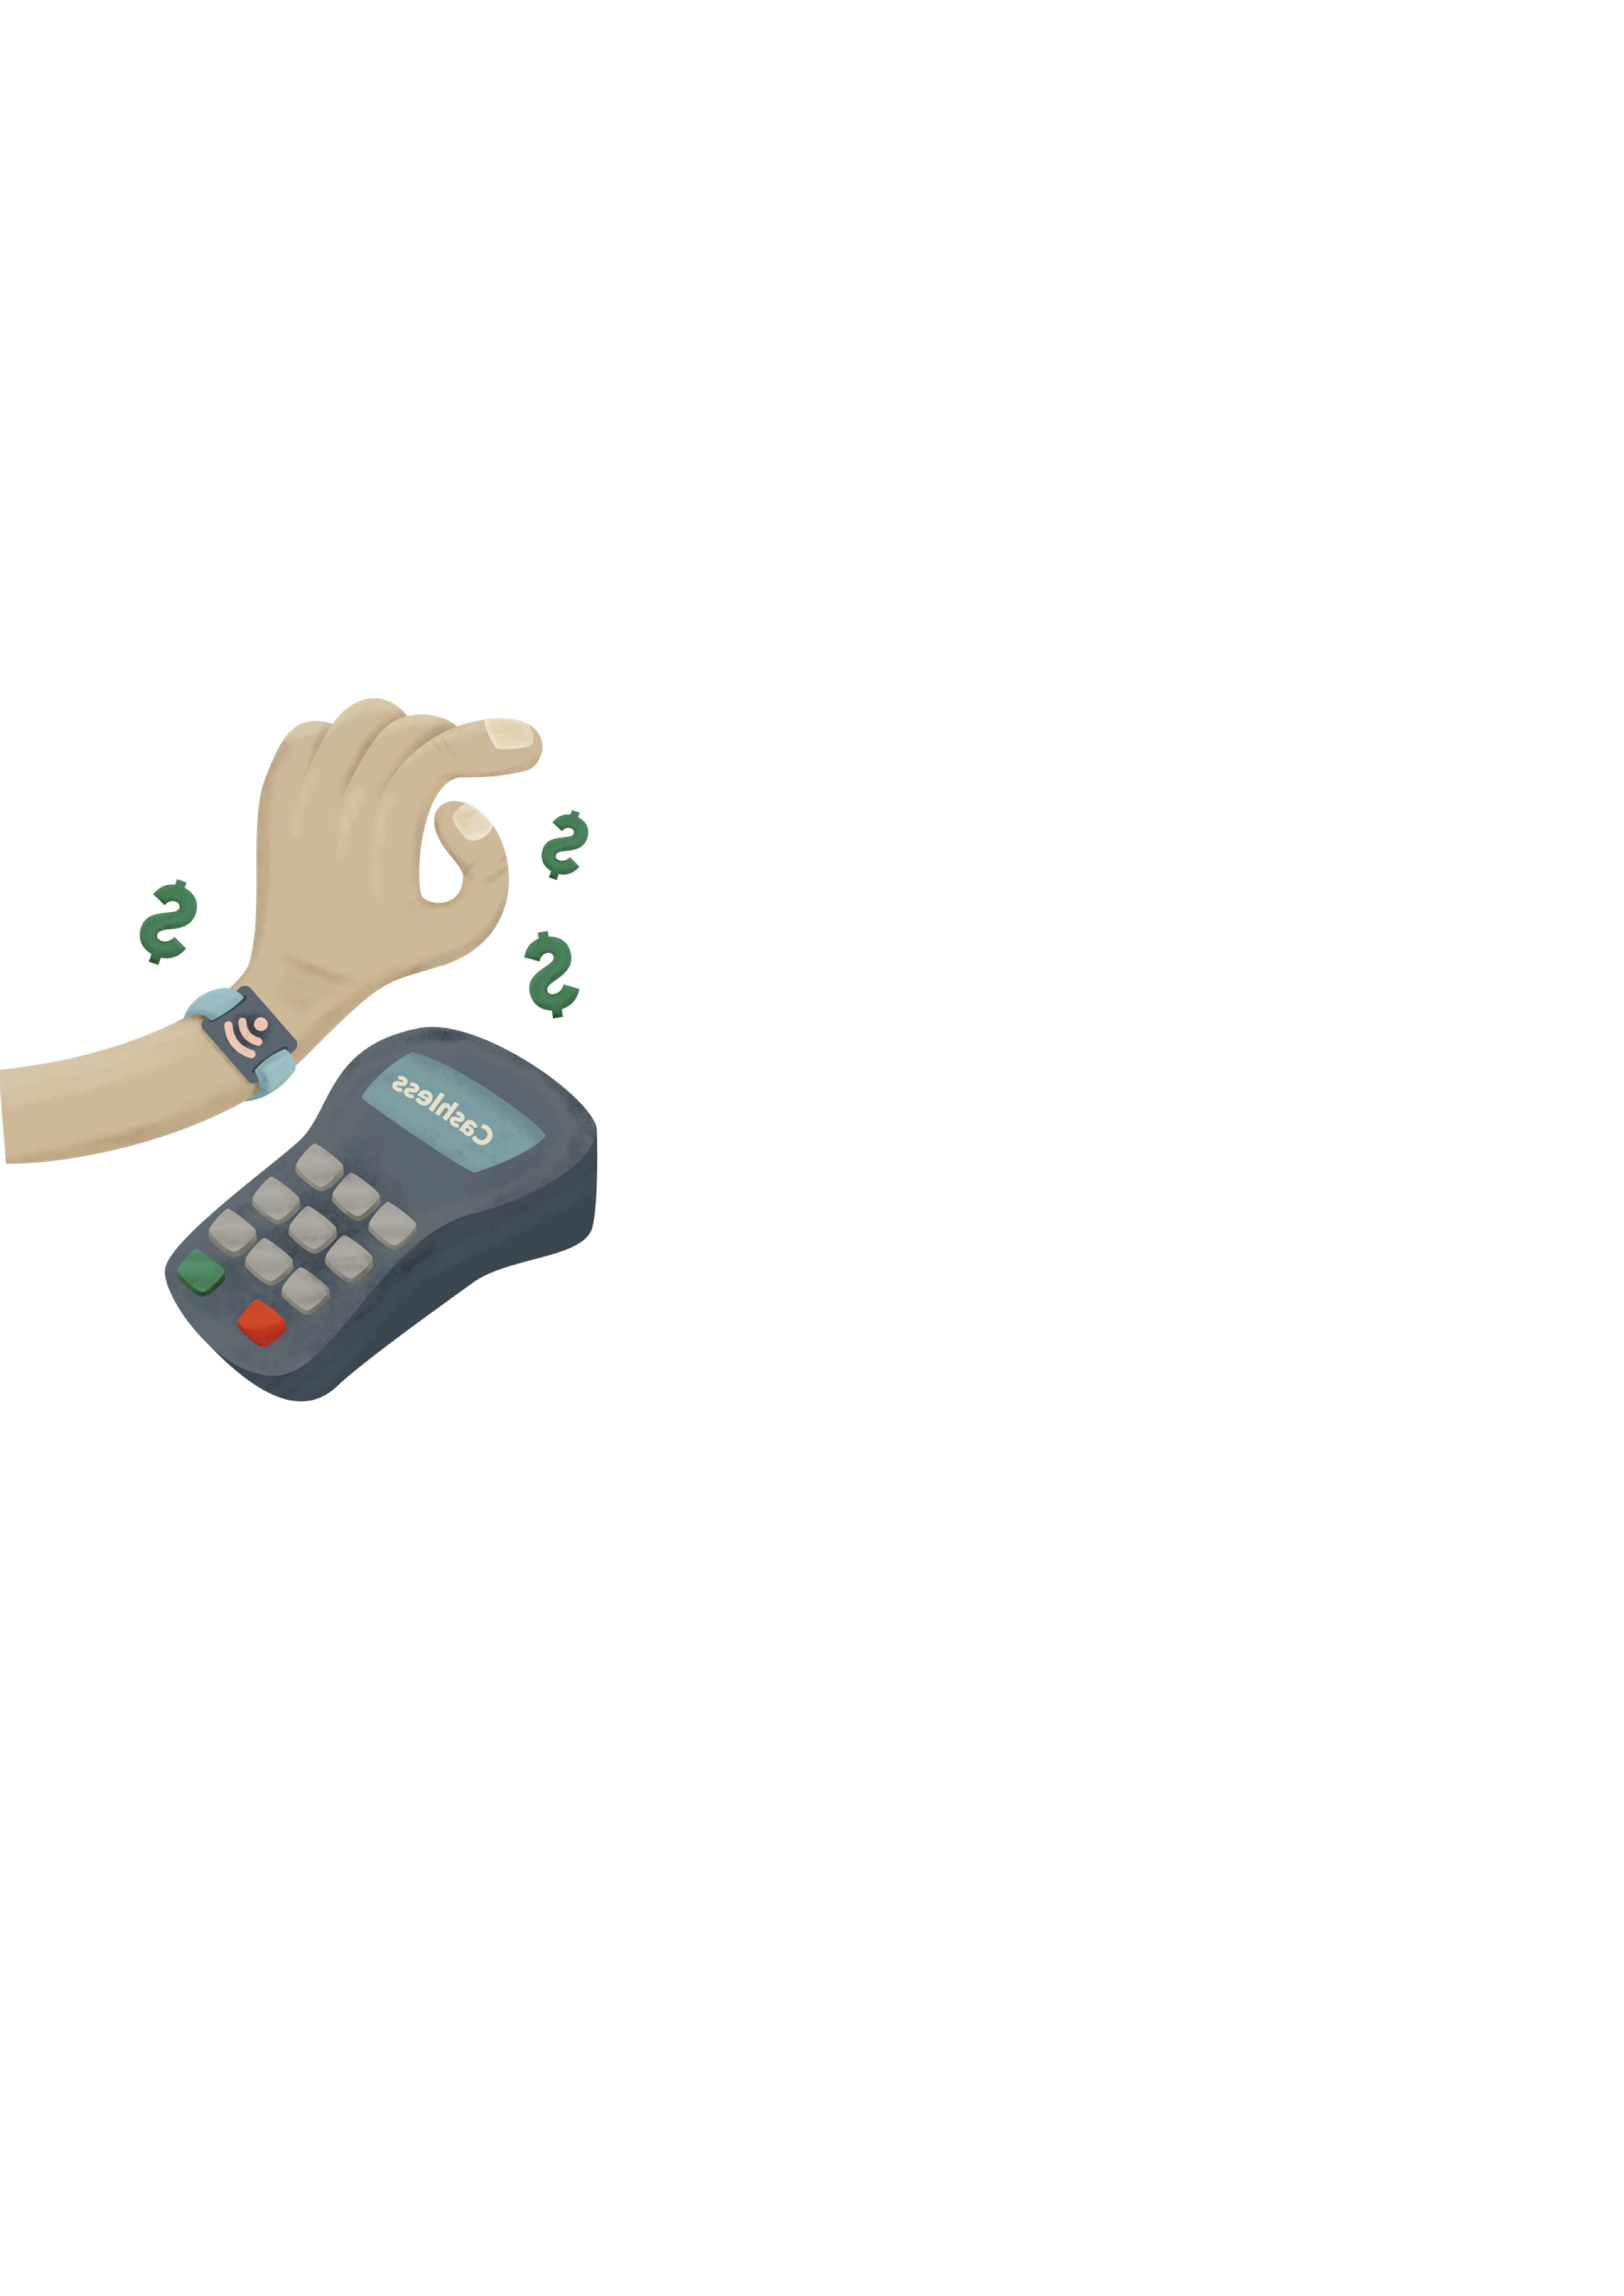
\includegraphics[width=\paperwidth,height=\paperheight]{billeder/Cashless_detaljeret_RGB.png}};
\section{Under Vagten}
\label{sec:intra-barvagten}

Under vagten er der diverse opgaver, der skal løses. 
Vi forventer I er høflige og møder gæsterne med smil og smuk ånd.

Husk at vaske eller spritte hænder af flere gange 
i løbet af vagten (sprit står på bordet i vognen).

For dem som står ude i køen, er der nogle opgaver vi skal have løst, inden folk kommer til 
en luge, og får sat deres kontanter ind, eller hvad de ellers skal.
Nogle gange skal folk ikke sætte kontanter ind, men skal blot have hjælp til:
\begin{itemize}
  \item At oprette sig på Cashless-appen
  \item At vide hvad man kan betale med inde på pladsen. Nogle gæster kommer måske for første gang, 
  og har ikke undersøgt, hvilke muligheder de har for betaling, inde på pladsen.
  Derfor er det for nogen nok at fortælle dem, at de blot kan betale med kort inde på pladsen.
  Dog er der nogle klare fordele ved at vælge at bruge Cashless-appen og sit armbånd.
  \begin{itemize}
    \item Det er ikke muligt at betale med MobilePay inde på pladsen, men det er muligt at 
    overføre penge med MobilePay fra Cashless-appen til armbåndet.
    \item Det er ikke usandsynligt at internettet på pladsen går ned i et øjeblik. Vi er 
    trods alt i en skov. Hvis det gør, er det nemlig kun muligt at betale med armbåndet.
    \item Det skal også siges, at det er en klar fordel for Smukfest, hvis gæsterne gør brug at 
    deres armbånd til betaling. For det første sparer Smukfest transaktionomkostinger, da i stedet for 
    at skulle betale for hvert enkelt småtransaktion, blot skal betale ét enkelt gebyr, når festivalen er omme. 
    Derudover hjælper det også, når gæsterne slå automatisk optankning til, og dermed ubesværet
    kan bruge penge inde på pladsen.
  \end{itemize}
\end{itemize}

\subsection{Cashless-appen}

Det er en god ide at I selv, inden I tager på jeres første vagt, opretter jer på
Cashless-appen, og tilknytter jeres armbånd, så I ved hvordan den fungerer. 
Ellers skal I nok hurtigt lære den at kende.
Gør dette så sent som muligt, da der kan komme opdateringer helt op til festivallen starter. \\

For at gæsterne kan sætte kontanter ind på deres armbånd, skal de have en konto på 
Cashless-appen (om de vil det eller ej), 
i tilfælde af at de ikke bruger alle deres penge, skal en konto tilknyttes til tilbagebetaling efter
festivalen. Hvis gæsterne har oprettet sig sidst år, behøver de det ikke igen i år.
Hvis gæsten ikke kan overbevises, eller ikke har mulighed for at oprette sig, er det kun muligt 
for dem at købe Walterkort, for deres kontanter (Se længere nede).

\subsection{Kasseapparater}
Vi har nogle særlige kasseapparater, lavet specifikt til vores arbejde, derfor er dette den bedste guide hertil. 
For at lære om kasseapparatets generelle funktioner, kan man læse betjeningsvejledningen fra 2019:
\begin{center}
  \small
  \href{https://memba.dk/media/478278/betjeningsvejledning-til-kasseterminal-2019-4.pdf}{https://memba.dk/media/478278/betjeningsvejledning-til-kasseterminal-2019-4.pdf}
\end{center}

Vi har tre kasseapparater til indsættelse af kontanter, og køb af Walterkort. Men derudover har vi også en 
enkelt kasse til udbetaling af kontanter for pant (Se længere nede).

\subsection{Kontanter}

Selvom at man står ude i køen og hjælper, og har nogle lidt andre opgaver, 
er det godt at vide hvad dem inde i pengekassen laver, 
så man ikke kommer til at henvise gæster de forkerte steder hen.

Pengekassens primære opgave er at veksle kolde kontanter (KUN SEDLER! Ingen mønter) til ``enheder'' på gæsternes armbånd, 
som de kan bruge inde på pladsen, til at købe kolde fadøl eller andet godt.

Det foregår således:
\begin{itemize}
  \item Tæl sedlerne
  \item Tryk `Indsæt beløb' på kasseapparatet, og bed gæsten om at bippe NFC-chippen på det armbånd pengene 
  skal lægges over på.
  \item En popup vil dukke frem, hvori beløbbet indtastes. 
  Check at beløbbet stemmer, og tryk `Ok'.
  \item Derefter printes en automatisk kvittering, som du kan tilbyde gæsten, eller smide ud.
  \item Sedlerne sorteres i bestikbakker under bordet, efter størrelse.
\end{itemize}

Hertil er der nogle ting man skal være opmærksom på.
\begin{itemize}
  \item Det vigtigt at pointere at det ikke er muligt for 
  os i pengekassen at trække enheder ud af gæsternes armbånd.
  Det betyder at man skal være sikker på, at det beløb man overfører til armåndet, 
  stemmer med hvad gæsten har afleveret. Et tip til at undgå det, er
  at lave saldocheck ved høje beløb eller ved mange sedler.
  Skulle det alligevel ske, skal der laves en sag på det, og udfyldes et
  udbetalingsbilag så vi kan håntere korrektioner.
  \item Gyldige sedler: På væggen i pengekassen hænger der billeder af de sedler vi tager imod, 
  hvis man skulle være i tvivl. Derudover skal de være intakte og ægte. 
  Det er dog ikke sådant at I skal checke hver enkelt seddel, da man typisk efter at have 
  hånteret et par sedler, kan mærke hvordan de skal føles.
  \item Beløbsgrænser: Max indbetaling på armbånd er \underline{15.000} kr. per dag. 
  De 15.000 kr. er ikke inkluderet, dvs. vi kan maks tage imod 14.950 kr. i sedler.
  \item Valuta: Kommer gæsten med udenlandsk valuta, tager vi også imod dem. Nedenfor 
  kan I se valutakurserne, for de sedler vi tager imod. Brug gerne en lommeregner til 
  at lave udregningen, og undgå fejl.
  \begin{itemize}
    \item Kursen på euro er 7,5. Dvs. 100 EUR bliver til 750 DKK.
  \end{itemize}
\end{itemize}

Som nævnt sorteres sedlerne i bestikbakker under bordet, en til hvert kasseapparat. 
Disse skal tømmes når de er ved at være fyldte, eller ved luk. Sedlerne må ikke blandes mellem kasser, 
da vi skal sørge for at alt bliver afstemt korrekt.

Den med ansvaret for at pakke poser, og levere dem til Banken ved siden af, gør således:
\begin{enumerate}
  \item Vælg 'Udskriv status' på kasseapparatet. En kvittering vil blive printet.
  \item Tag kvitteringen og sedlerne fra bakken med hen til indhakket ved indgangen, til vognen
  \item Tag et lyserødt bilag (tre sider), og skriv nedstående oplysninger på forsiden:
  \begin{itemize}
    \item Dato
    \item Klokkeslet
    \item Pose nr.
    \item Kassenr.
    \item Beløbet på afstemningskvitteringen
    \item Underskrift
  \end{itemize}
  \item Tag en pengepose, og kom disse ting ned i posen:
  \begin{itemize}
    \item Alle sedler fra kassen, sorteret efter størrelse, så det er hurtigere for dem i Banken at 
    tælle dem. 
    \item Evt. udbetalingsbilag i tilfælde af fejlekspedition.
    \item Til sidst rives en side fra gennemslagspapiret af, og lægges med forsiden udaf ind i pengeposen.
  \end{itemize}
  \item Pengeposen lukkes.
  \item I år indfører vi kvittering for afleveringen, dvs. der skal kvitteres for aflevering og modtagelse 
  af pengeposer mellem Pengekasse og Bank.
  Kvitteringen hedder ``pengelisten'', så vi dagligt laver en opgørelse over alle pengeposer som laves i pengekassen. 
  På pengelisten skrives hver pengepose til banken op med oplysninger om: 
  \begin{itemize}
    \item Dato
    \item Klokkeslet
    \item Pose nr.
    \item Kassenr.
    \item Underskrift
  \end{itemize}
\end{enumerate}

\subsection{Waltherkort}
Waltherkort er et supplement til betaling med armbånd eller dankort på pladsen.
Gæsterne kan købe dem med kort eller kontanter, og kortene er foruddefineret med et fast beløb:
\begin{itemize}
  \item 500 kr.
  \item 1000 kr.
  \item 2000 kr.
\end{itemize} 

Nogle forskellige virksomheder har forudbestilt Walterkort til deres medarbejdere, 
som de kommer og henter hos os. 
De ligger i hver deres kurvert, og på en tilhørende liste, findes det tilknyttede navn 
og hvad der står på kurverten.
Da Walterkortene er forudbetalte SKAL den person 
som står til at skulle hente kortene, være den der henter dem.
Walterkortene er talt på forhånd, men ofte vil gæsterne gerne tælle efter, 
og checke at de har de rigtige beløb.
Derudover skal gæsten skrive under på at de har hentet kortene.

Der vælges en luge tættest ved Walterkortene, til håndtering hertil.

De Walterkort gæsterne har bestilt på forhånd har blanke bagsider, modsat dem vi sælger,
som har en guide på bagsiden, til at få pengene retur efter festivalen.
Blanke bagsider kan IKKE byttes til andre af samme værdi. Kun hvis de har en guide på bagsiden 
kan de godt, men vi vil helst undgå det.

Opstår der problemer med Walterkort, som I ikke kan løse, kan I altid kontakte mig (Anders), eller Rikke Møller 
inde i banken ved siden af. 
% Snak i formandsreceptionen I stedet for i lågerne

\subsection{Pantkassen}

Det er muligt at aflevere pant på Smukfest, men disse steder indbetaler kun enheder på pantsamlernes armbånd.
Derfor kan der være nogle der vil have pengene kontant. Hertil har vi et særligt kasseapparat.

Pantkassen står fast længst inde i vognen, op af væggen, og tages frem når vi udbetaler pant.
Vi udbetaler kun pant indenfor åbningstiderne, onsdag til lørdag 10-12, og søndag 10-18.

Vi udbetaler kun i sedler, så hvis beløbet ikke helt kan udbetales, rundes der ned 
til nærmeste seddel, og resten bliver ikke udbetalt. 
Pant har sin egen kassebeholdning og må ikke blandes med pengene i de andre kasser, 
da de skal opgøres separat. Mangler der penge til pant skal der hentes pengepose i banken. 
Pengelisten til afstemning skal også udfyldes for pantkassen.

Sådan udbetales pant på terminalen: 
\begin{enumerate}
  \item Scan gæstens armbånd med saldotjek (f.eks. 5.211 kr.).
  \item Indtast 5.200 på terminalen.
  \item Tæl pengene fra pantkassen.
  \item Scan armbåndet igen og vælg ``NFC udbetaling''.
\end{enumerate}

%\tikz[remember picture,overlay] 
%\node[opacity=0.2,inner sep=0pt] at (current page.center)
%{
\includegraphics[width=\paperwidth,height=\paperheight]{billeder/Burger.png}};

\tikz[remember picture,overlay] 
\node[opacity=0.2,inner sep=0pt] at (current page.center)
{
\includegraphics[width=\paperwidth,height=\paperheight]{billeder/Cashless_simpel_RGB.png}};

\begin{enumerate}
  \item[4.] Bekræft `Ok'.
  \item[5.] Tæl pengene 5.200 kr. til gæsten.
\end{enumerate}

Derudover skal man være opmærksom på at man max må udbetale pant for \underline{8.000} kr. per dag.

\subsection{Mad}

Under vagten skal der selvfølgelig være tid til at smutte ud og finde noget mad, og få et 
pusterum, væk fra gæsterne. Lige uden for vognen er et sofahjørne, hvor man kan slappe af i 
sin pause, så man også giver plads til dem inde i vognen.
I forhold til mad er der bestil morgenmadspakker til afhentning i Vores Bar. 
Derudover kan man købe og lave sine egne toast, i det lille køkken bag ved armbåndssupport, 
til en skarp pris. Under vagten vil der også være slik og søde sager, man kan snacke.

Søger man noget mere mættende, kan man smutte ind på pladsen og gøre brug af de boder man har lyst til der.
Hertil kan man bruge af de 300 enheder man har fået sat ind på sit medhjælperarmbånd. Et tip til at få mest 
ud af sine enheder, er selvfølgelig at gå i Vores Bar, hvor man kan få nogle af de samme ting, bare til en 
skarpere pris.

\subsection{Drikke}

Det er også vigtigt at få nok at drikke.
Flere steder kan man finde vandposter, til at fylde sin drikkedunk eller kop op med.
Er man til kaffe, kan dette også findes i det lille køkken bag ved armbåndssupport.
Derudover er der køleskabe i vores bagområde, med forskellige sodavand, til fri 
afbenyttelse. \\

Vent dog med at nyde alkohol til efter vagten. Nu har vi med mange kontanter at gøre, 
så det forventes også I kan håntere det seriøst. 
Møder man fuld op eller bliver det under vagten, kan det have konsekvenser, og i 
værste fald et klippet armbånd.

\subsection{Andet}
\label{sec:intra:andet}

Nu ved I hvilke generelle opgaver vi har og løser, men det betyder ikke 
at der ikke kan komme andre opgaver op. Her handler det om at hjælpe gæsterne 
bedst muligt, ved bl.a. at henvise dem til de rigtige.

Er der fejl på gæstenes armbåndschip, henviser vi til informationen i Sherwood - tag gæsterne ``i hånden'' 
og lav en god overlevering.
%Vi har erfaring med at gæster nogle gange kommer retur, efter de har fået at vide fra 
%armbåndsupport, at det er os der kan hjælpe dem, hvor vi er nødsaget til at gå med dem derhen, 
%og forklare problemet. Dette skyldes for det meste, fordi armbåndsupport ikke helt 
%ved hvad det er vi har mulighed for at hjælpe med, og tror vi kan noget andet end vi 
%rent faktisk kan.

% Hvor mange poser har vi pakket og sendt afsted + beløb 
